% !TeX root = ../../thesis.tex
\chapter{This is chapter2}\label{ch:chapter2}

\begin{minipage}[b]{0.6\textwidth}
    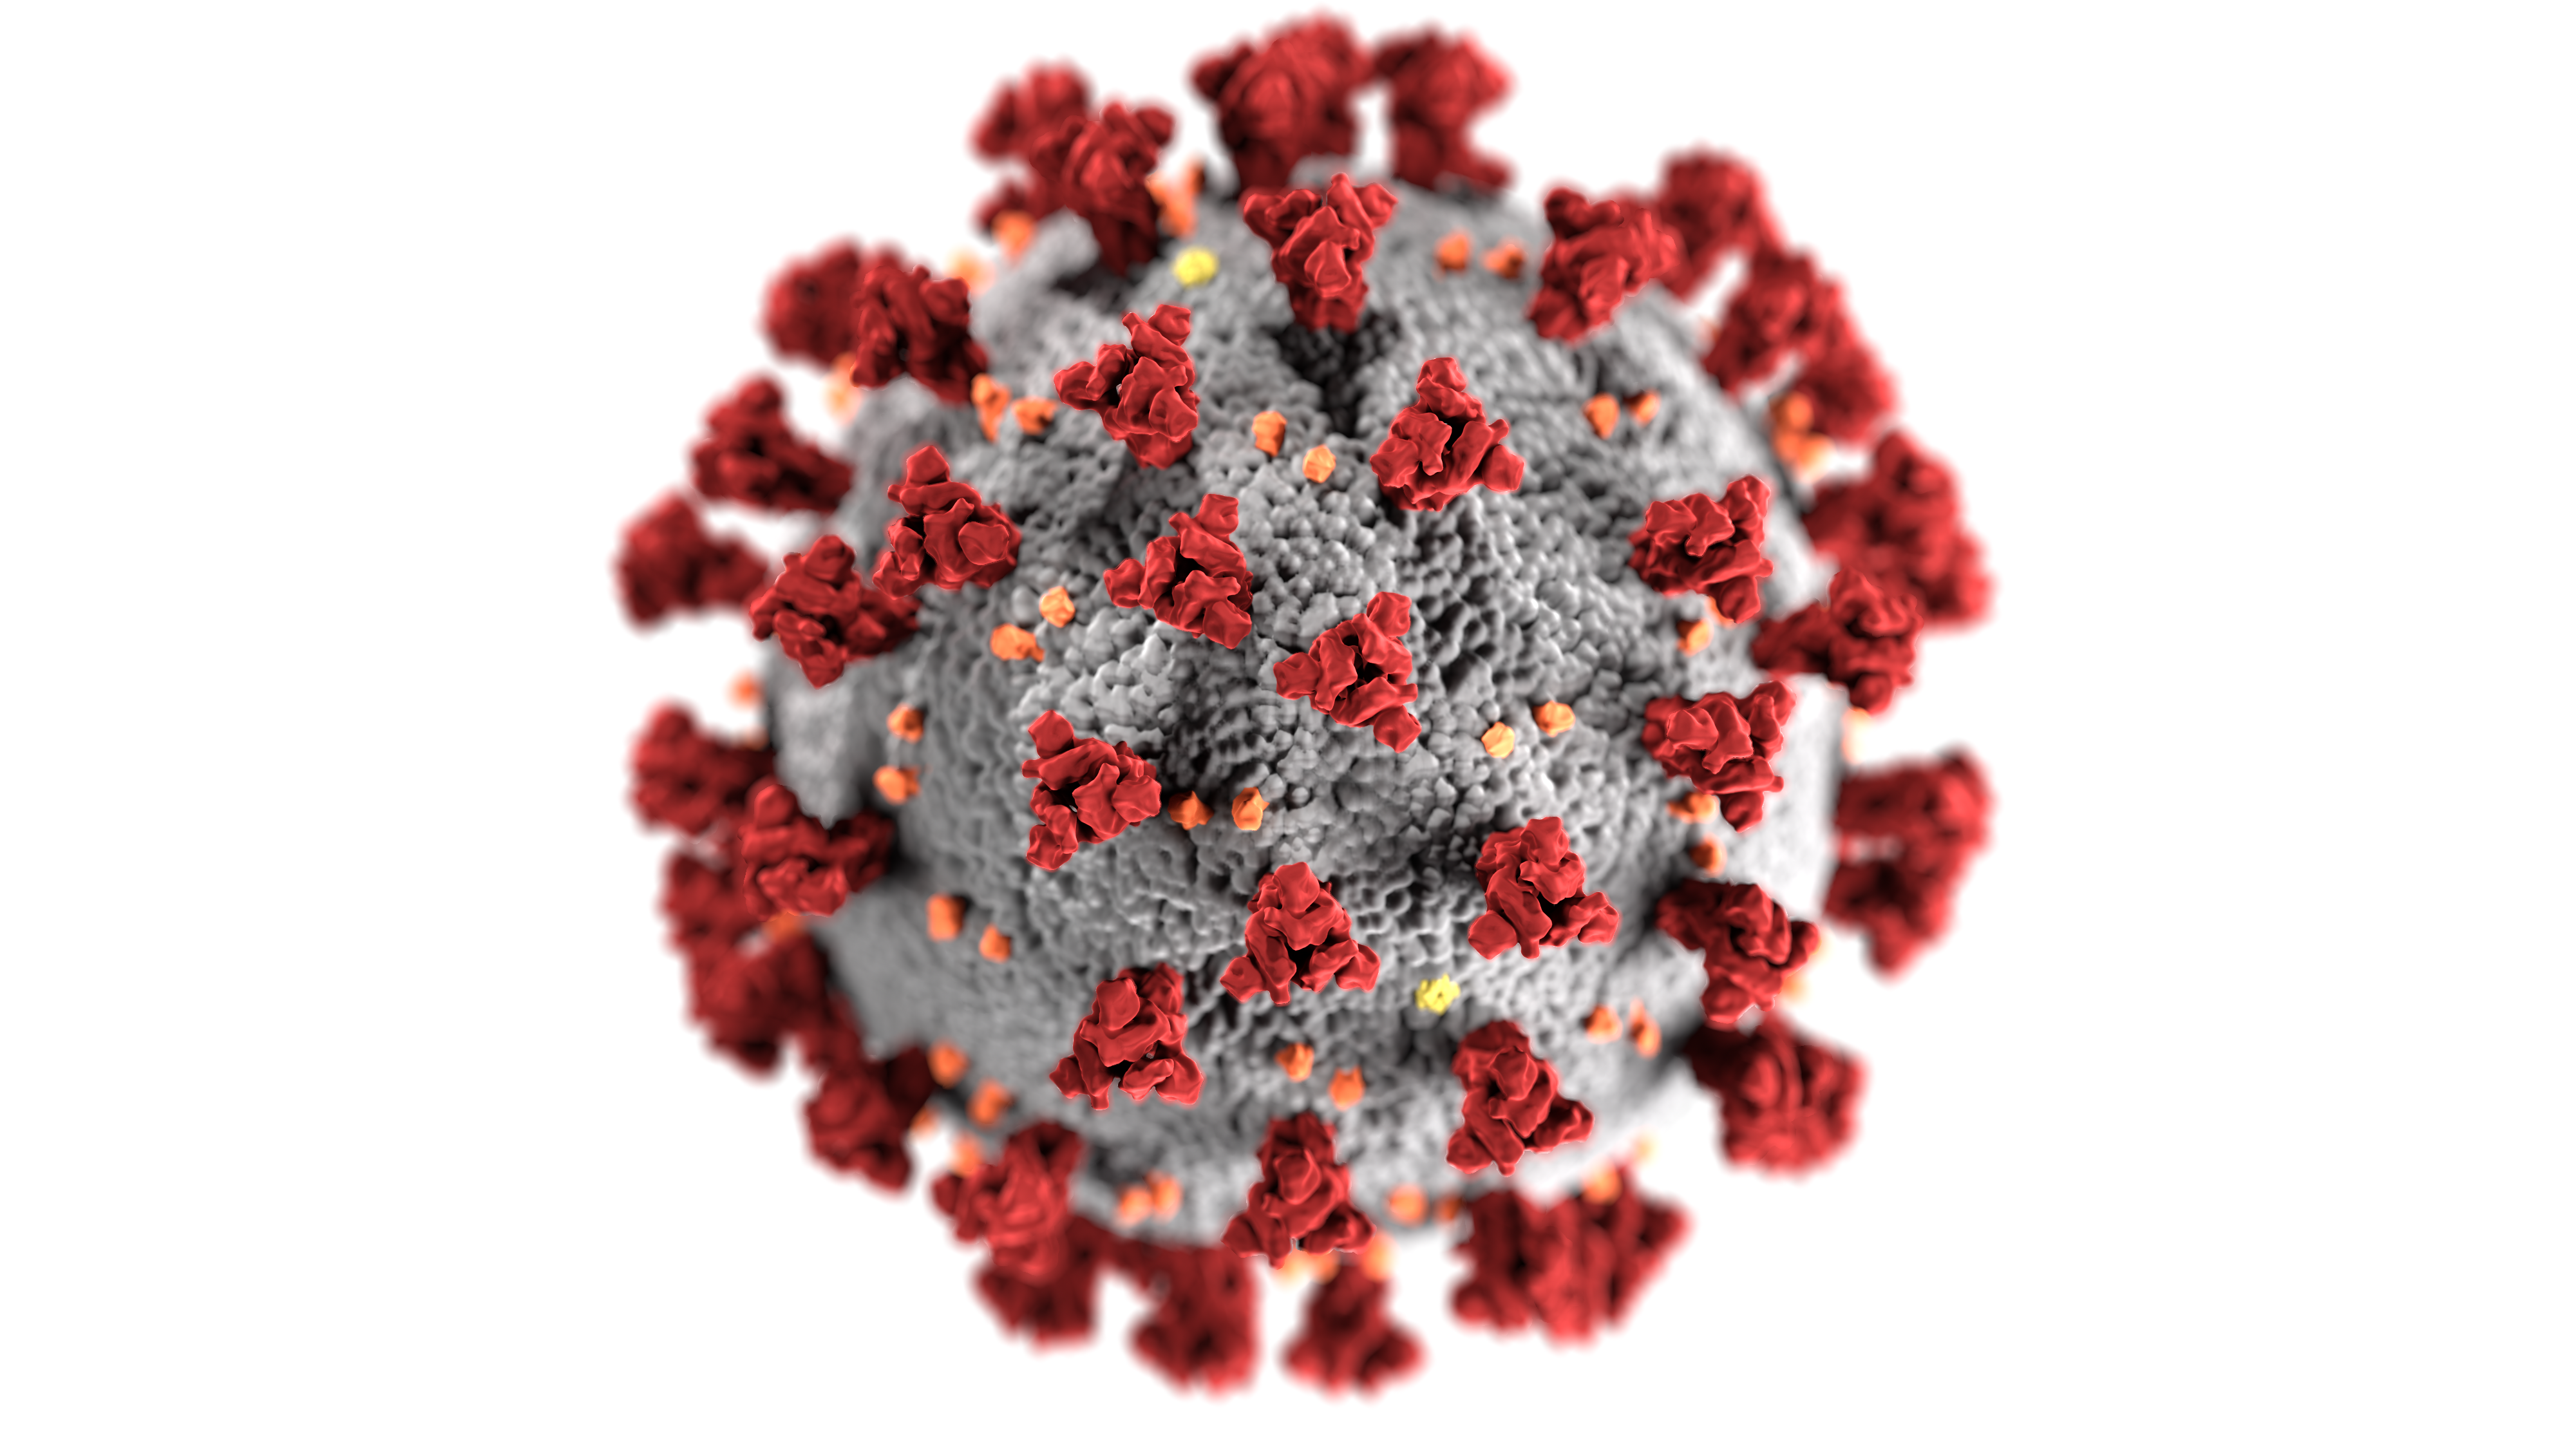
\includegraphics[width=\textwidth]{title} % Note: image needs to be cropped and faded
    % https://phil.cdc.gov/Details.aspx?pid=23312
  \end{minipage}
  \hfill
  \begin{minipage}[b]{0.35\textwidth}
    \footnotesize
    \begin{flushright}
      \textit{``A learning experience\\is one of those things that says,\\'You know that thing\\you just did?\\Don't do that.'\thinspace''} \\
      --- Douglas Adams, \\The Salmon of Doubt
    \end{flushright}
    \vspace{2cm}
  \end{minipage}
  
  \clearpage

\ldots




%%%%%%%%%%%%%%%%%%%%%%%%%%%%%%%%%%%%%%%%%%%%%%%%%%
% Keep the following \cleardoublepage at the end of this file, 
% otherwise \includeonly includes empty pages.
\cleardoublepage

% vim: tw=70 nocindent expandtab foldmethod=marker foldmarker={{{}{,}{}}}
